\section{Infinite Series}
Well here's an interesting question.
\begin{center}
\emph{What does it mean to add up infinitely many numbers?}

\parindent \parindent -Lots of people
\end{center}

We provide the most commonly used modern \infiniteseries{definition}.

\begin{definition}{Infinite Series, Convergence, and Divergence}
Let $a_n$ be a sequence of real numbers.  Then the \emph{infinite sum} of all terms of $a_n$ is defined to be the limit of partial sums $A_N$.  That is, 
$$\sum_{n=0}^\infty a_n = \lim_{N\rightarrow \infty} A_N = \lim_{N\rightarrow \infty} \sum_{n=0}^N a_n. $$
If the limit exists, we say the \conv{infinite series} \emph{converges} to the value of the limit.  If the limit is infinity or does not exist, then we say the \divergence{infinite series} \emph{diverges}. 
\end{definition}

The idea is simple; if you want to add up infinitely many numbers, a good place to start is by just adding up finitely many of them.  However, if you only add up finitely many, your answer has some error to it.  If you want that error to go down, add up more and more of them!  The limit of the values of these partial sums will be the exact answer.

\begin{exercise}{The Return of the Discrete/Continuous Analogy \Coffeecup \Coffeecup \Coffeecup} In what way is the definition of an infinite series analagous to the definition of a horizontally unbounded improper integral?
    \solushun{
        In the same way that the definition of the infinite series involves taking the limit as the last term approaches infinity, the definition for a horizontally unbounded improper integral also involves taking the limit of the upper bound of integration: $ \int_{a}^\infty f(x)\dif x = \lim_{c \rightarrow \infty} \int_{a}^c f(x)\dif x. $ \\
    }{.5in}
\AnswerKeyEntry{Think about an integral of the form $\intop_{x=0}^{x=\infty}f(x)\dif x $.  How does one handle that infinity in the bounds?}
\end{exercise}

\begin{exercise}{The Definitions in Words \Coffeecup \Coffeecup}
We have defined three very important interconnected structures: 
\begin{itemize}
\item A sequence $a_n$.
\item A sequence of partial sums $A_N$.
\item An infinite series $\sum_{n=0}^\infty a_n$.
\end{itemize}
Describe in words how the three structures are related and are built from one another.
    \solushun{
        Taking the sum of some consecutve elements of the sequence $a_n$ produces the partial sums $A_N$. If we take an infinite number of the elements of $a_n$ and sum them, we generate the infite series $\sum_{n=1}^\infty$, which is equivalent to taking the limit $\lim_{N\to\infy}A_N$.\\
    }{1in}
 \end{exercise}
 
 \subsection{Zeno's \Zeno{Paradox}, Resolution, and Consequences}\label{infser} 
 
The next example is traceable back to the writings of Aristotle in the third century BC!  Specifically, he states Zeno's Paradox of \emph{Dichotomy} as: \begin{center}
\emph{That which is in locomotion must arrive at the half-way stage before it arrives at the goal.}
\end{center}

% https://en.wikipedia.org/wiki/Zeno%27s_paradoxes#/media/File:Zeno_Arrow_Paradox.png
% and the little rules under ``Suppose Homer...''
% https://en.wikipedia.org/wiki/Zeno%27s_paradoxes
	\begin{center}
		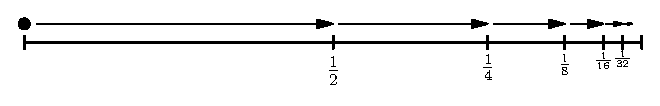
\includegraphics[width=400pt]{ChapterSeqSer/Figures/zeno.eps}
	\end{center}
    %This one is super simple and we can discuss modifying it to something better...

This was meant to be a ``proof'' that an object (say an arrow in flight) could never reach its target.  This paradox is resolved with our notion of infinite series. 

\begin{exercise}{A Classic Infinite Series \Coffeecup \Coffeecup}
Consider the sequence $\frac{1}{2},\frac{1}{4},\frac{1}{8},\frac{1}{16},\ldots$.  This can be interpreted as the sequence of distances the arrow must travel in the Dichotomy paradox (supposing it was fired one meter from its target and all lengths are measured in meters).  Since it were fired from one meter away, we expect that the total distance traveled is one.

\begin{itemize}
\item Find an explicit formula $a_n$ that describes the sequence above.
    \solushun{
        $a_n=\frac{1}{2^{n+1}}$.\\ 
    }{.5in}
\item Compute the corresponding sequence of partial sums $A_N$. 
    \solushun{
        Taking the Geometric Series Formula, with first term $\frac{1}{2}$ and common ration $\frac{1}{2}$, we get
        $$A_N=\frac{1}{2}\cdot \frac{1-\left(\frac{1}{2}\right)^{n+1}}{1-\frac{1}{2}}=\frac{1}{2}\cdot \frac{1-\frac{1}{2^{n+1}}}{\frac{1}{2}}=1-\frac{1}{2^{n+1}}.$$
    }{.5in}
\item Evaluate the infinite sum $$\frac{1}{2}+\frac{1}{4}+\frac{1}{8}+\frac{1}{16}+\cdots $$
by taking the limit of the sequence of partial sums.  Verify the total is in fact one.
        \solushun{
            $$\lim_{N\to\infty}1-\frac{1}{2^{N+1}}=1-\lim_{N\to\infty}\frac{1}{2^{N+1}}=1-0=1.$$
        }{1in}
\end{itemize}

\AnswerKeyEntry{The sequence is $a_n=\frac{1}{2^{n+1}}$.  Since this is a geometric sequence, the finite geometric series formula can be applied to then find the sequence of partial sums $A_N$.}
\end{exercise}

In the above case, we were able to provide a \Zeno{resolution} for the paradox and verify the total with our geometric series formula, but the answer was not particularly surprising.  Here is a more interesting example! 

\begin{exercise}{An \alternatingseries{Alternating Geometric Series} \Coffeecup \Coffeecup \Coffeecup}\label{alternatebug}
Suppose a bug moves forward half a meter.  It then moves backwards one-fourth of a meter. It then moves forward one-eighth of a meter.  It then moves backwards one-sixteenth of a meter.  This pattern of moving forwards, then backwards, by half the previous distance each time, continues forever.  At the end of time, where does the bug end up?

To solve this problem, we notice that it is equivalent to adding up all terms in the sequence $\frac{1}{2},-\frac{1}{4},\frac{1}{8},-\frac{1}{16},\cdots $.  Following the method of Example \ref{Toemato}.\ref{UsedToBePlicit},
this sequence can be expressed as a geometric sequence with initial term $a_0=\frac{1}{2}$ and common ratio $r=-\frac{1}{2}$ as follows: $$ a_n=\frac{1}{2}\left( -\frac{1}{2} \right) ^n.$$
\begin{itemize}
\item Let $A_N=\sum_{n=0}^N a_n$ be the sequence of partial sums.  Find a formula for $A_N$. 
    \solushun{
        Since this is a geometric series, we again use the Geometric Series Formula:
        $$A_N=\frac{1}{2}\cdot\frac{1-\left(-\frac{1}{2}\right)^{N+1}}{1-\left(-\frac{1}{2}\right)}=\frac{1}{2}\cdot\frac{1-\left(-\frac{1}{2}\right)^{N+1}}{\frac{3}{2}}=\frac{1-\left(-\frac{1}{2}\right)^{N+1}}{3}.$$
    }{1in}
\item  Compute $ \sum_{n=0}^{5} a_n.$
    \solushun{
        $$A_5=\frac{1-\left(-\frac{1}{2}\right)^{5+1}}{3}=\frac{1-\left(-\frac{1}{2}\right)^{6}}{3}=\frac{1-\frac{1}{64}}{3}\approx 0.4219.$$
    }{1in}
\item  Compute $ \sum_{n=0}^{10} a_n.$
    $$A_{10}=\frac{1-\left(-\frac{1}{2}\right)^{10+1}}{3}=\frac{1-\left(-\frac{1}{2}\right)^{11}}{3}=\frac{1+\frac{1}{2^{11}}}{3}\approx 0.3335.$$
\item Compute $ \sum_{n=0}^{\infty} a_n$ from the definition of an infinite series.
    \solushun{
        Take the limit of $A_N$ as $N$ approaches infinity.
        $$\lim_{N\to\infty} A_N=\lim_{N\to\infty} \frac{1-\left(-\frac{1}{2}\right)^{N+1}}{3}=\frac{1-\left(\lim_{N\to\infty}\left(-\frac{1}{2}\right)^{N+1}\right)}{3}=\frac{1}{3}.$$
    }{1in}
\end{itemize}

So, where does the bug end up?
    \solushun{
        It ends up one-third of a meter forward from where it started.\\
    }{.5in}
\AnswerKeyEntry{It ends up one-third of a meter forward from where it started.}
\end{exercise}
\subsection{Infinite Geometric Series}\label{Geometrickery}
The notion of an infinite series can be used to give a rigorous interpretation to the infinite decimal expansions as well! 

\begin{exercise}{Repeating Decimal Expansion \Coffeecup \Coffeecup }\label{ThreeBar}

\begin{itemize}
\item Notice that the decimal expansion 0.333 can be written as a geometric series with three terms and common ratio $1/10$ using the definition of place value.  In particular, $$ 0.333=\frac{3}{10}+\frac{3}{100}+\frac{3}{1000}.$$ Compute its value via the finite geometric series formula.

    \solushun{
        This is a geometric series with first term $\frac{3}{10}$ and common ration $r=\frac{1}{10}$, and $3$ terms. By the geometric series formula we get 
        $$\frac{3}{10}\cdot\frac{1-\frac{1}{10^3}}{1-\frac{1}{10}}=\frac{3}{10}\cdot\frac{1-\frac{1}{1000}}{\frac{9}{10}}=\frac{\frac{999}{1000}}{3}=\frac{333}{1000}=0.333$$.
    }{1in}

\item Write 0.3333 as a geometric series with four terms and common ratio 1/10.  Compute its value via the finite geometric series formula.

    \solushun{
        $$ 0.3333=\frac{3}{10}+\frac{3}{100}+\frac{3}{1000}+\frac{3}{10000}$$.
        Evaluating this with the geometric series formula is almost exactly the same as the previous problem.
        $$\frac{3}{10}\cdot\frac{1-\frac{1}{10^4}}{1-\frac{1}{10}}=\frac{3}{10}\cdot\frac{1-\frac{1}{10000}}{\frac{9}{10}}=\frac{\frac{9999}{10000}}{3}=\frac{3333}{10000}=0.3333$$.
    }{1in}

\item Write 0.33333 as a geometric series with five terms and common ratio 1/10.  Compute its value via the finite geometric series formula.

    \solushun{
        $$ 0.33333=\frac{3}{10}+\frac{3}{100}+\frac{3}{1000}+\frac{3}{10000}+\frac{3}{100000}$$.
        Repeat the process above.
        $$\frac{3}{10}\cdot\frac{1-\frac{1}{10^5}}{1-\frac{1}{10}}=\frac{3}{10}\cdot\frac{1-\frac{1}{100000}}{\frac{9}{10}}=\frac{\frac{99999}{100000}}{3}=\frac{33333}{100000}=0.33333$$.
    }{1in}

\item Write $$ \underbrace{0.3333 \ldots 3}_{n \textup{ threes}} $$ as a geometric series with $n$ terms and common ratio 1/10.  Compute its value in terms of $n$ via the finite geometric series formula.

    \solushun{
        $$ 0.33333\ldots3=\frac{3}{10}+\frac{3}{100}+\frac{3}{1000}+\frac{3}{10000}+\frac{3}{100000}+\cdots+\frac{3}{10^n}$$.
        Repeat the process above.
        $$\frac{3}{10}\cdot\frac{1-\frac{1}{10^{n+1}}}{1-\frac{1}{10}}=\frac{1-\frac{1}{10^{n+1}}}{3}.$$
    }{1in}

\item Take the limit as $n$ approaches infinity of your formula from the previous part to prove that ''point three repeating" really does equal one-third.

    \solushun{
        $$\lim_{n\to\infty}\frac{1-\frac{1}{10^{n+1}}}{3}=\frac{1-\lim_{n\to\infty}\left(\frac{1}{10^{n+1}}\right)}{3}=\frac{1}{3}.$$
    }{1in}
\end{itemize}
\end{exercise}

We can generalize the previous examples.  Notice in all cases, the geometric series formula let us calculate an explicit formula for the sequence of partial sums.  As long as the common ratio $|r|<1$, the limit as $n\rightarrow \infty$ will exist, as the $r^{N+1}$ term will go to zero and we will be left with just $a_0\frac{1}{1-r}$.  This brings us to the \emph{infinite geometric series} formula (also sometimes just referred to as the geometric series formula).

\begin{theorem}{\geometricseries{Infinite} Geometric Series Formula }
If $a$ and $r$ are real numbers and $|r|<1$, then $$a+ar+ar^2+ar^3+\cdots=\frac{a}{1-r}.$$  
\end{theorem}

Notice in the above formula, the number $a$ represents the first term of the series and $r$ represents the common ratio.

\begin{example}{A Messier Repeating Decimal Expansion}
Suppose we wish to write the repeating decimal $$1.\overline{615384} $$ as a fraction. We repeat (heh) the method of Exercise \ref{Geometrickery}.\ref{ThreeBar}, where we use base-ten place value to express the decimals as sums of terms with common ratio equal to a negative power of ten.
\begin{align*}
1.\overline{615384}&=1.615384615384615384\ldots \\
&=1+\frac{615384}{10^6}+\frac{615384}{10^{12}}+\frac{615384}{10^{18}}+\cdots
\end{align*}
The very first term, 1, clearly does not fit the pattern given by the rest of the terms.  So, we won't worry about that term, and instead just work on evaluating the rest while we leave the 1 out front.  The rest of the terms form an infinite geometric series with initial term $a=\frac{615384}{10^{6}}$ and common ratio $r=\frac{1}{10^6}$.  We now apply the infinite geometric series formula, noting that $r$, being one over a million, is comfortably between -1 and 1 as required.  Note that we resolve the compound fraction below by multiplying the top and bottom by $10^6$.
\begin{align*}
1.\overline{615384}
&=1+\frac{\frac{615384}{10^6}}{1-\frac{1}{10^6}} \\
&=1+\frac{615384}{10^6-1}\\
&=1+\frac{615384}{999999}\\
&=1+\frac{8}{13}\\
&=\frac{21}{13}\\
\end{align*}
\end{example}

\begin{exercise}{Using the Geometric Series Formula \Coffeecup \Coffeecup}

 Consider the following series: $$ \sum_{n=5}^{\infty} \frac{3^n}{2^{2n+1}}$$
\begin{itemize}
\item  Write out the first few terms of the above series.  That is, expand the sigma notation by plugging in $n=5,6,7,8,\ldots$ and evaluating the summand in each case.

    \solushun{
        \begin{center}
        \begin{tabular}{|c|c|l|c|} \hline
            $n$ & $a_n$ & $A_n$ & Total \\ \hline
            $5$ & $\frac{3^5}{2^{11}}$ & $\frac{3^5}{2^{11}}$ & $\approx 0.1187$ \\
            $6$ & $\frac{3^6}{2^{13}}$ & $\frac{3^5}{2^{11}}+\frac{3^6}{2^{13}}$ & $\approx 0.2076$ \\
            $7$ & $\frac{3^7}{2^{15}}$ & $\frac{3^5}{2^{11}}+\frac{3^6}{2^{13}}+\frac{3^7}{2^{15}}$ & $\approx 0.2744$ \\
            $8$ & $\frac{3^8}{2^{17}}$ & $\frac{3^5}{2^{11}}+\frac{3^6}{2^{13}}+\frac{3^7}{2^{15}}+\frac{3^8}{2^{17}}$ & $\approx 0.3244 $ \\
        \end{tabular}
        \end{center}
    }{1in}

\item  Is the above series geometric?  Explain why or why not.  If so, what is the common ratio $r$?  What is the first term $a$?

    \solushun{
        Yes it is, because each term is a ratio of the last term. The common ratio $r=\frac{3}{4}$ and the first term is $\frac{3^5}{2^{11}}$.\\ 
    }{1in}

\item  Find the value of the above series.
    
    \solushun{
        Plugging what we have into the infinite geometric series formula, we get
        $$ \sum_{n=5}^{\infty} \frac{3^n}{2^{2n+1}}=\frac{\frac{3^5}{2^{11}}}{1-\frac{3}{4}}=\frac{\frac{3^5}{2^{11}}}{\frac{1}{4}}=\frac{3^5}{2^{11}}\cdot 4=\frac{3^5}{2^9}\approx 0.4746.$$

    }{1in}

\end{itemize}
\AnswerKeyEntry{Yes, the series is geometric with initial term $\frac{3^5}{2^{11}}$ and common ratio $3/4$.  The infinite series totals to $
\frac{3^5}{2^9}$.}
\end{exercise}
\begin{exercise}{Not Using the Geometric Series Formula \Coffeecup}
Explain why the following calculation is not valid according to our definition of infinite series:
\begin{align*}
1+2+2^2+2^3+2^4+\cdots &=\frac{1}{1-2} \\
&=-1
\end{align*}
\AnswerKeyEntry{Think about what the value of $r$ would be for that series.  What restrictions did we have on $r$ in the statement of the infinite geometric series formula?}
\end{exercise}
\begin{exercise}{The Bouncing Ball \Coffeecup \Coffeecup}
	\begin{center}
		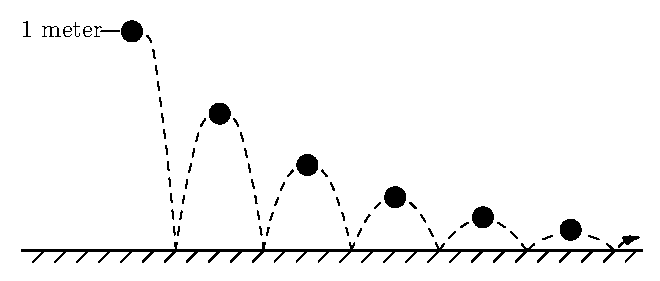
\includegraphics[width=300pt]{ChapterSeqSer/Figures/ball.eps}        
	\end{center}
    A magical bouncy ball is bounced from a height of 1 meter.  On each bounce, it always rebounds to exactly five-eighths of the height it fell from.  What is the ball's total vertical distance traveled from now until the end of time?
    \vspace*{1in}
    \AnswerKeyEntry{$1+2\frac{5}{8}+2\left(\frac{5}{8}\right)^2+2\left(\frac{5}{8}\right)^3+\cdots=1+2\frac{5/8}{1-5/8}=1+2\frac{5/8}{3/8}=13/3=4.\overline{3}$ meters.}
\end{exercise}

\begin{exercise}{Evaluating Another Infinite Series \Coffeecup \Coffeecup}

Consider the constant sequence $ a_n=2$.  Now consider the corresponding infinite sum: $$ \sum_{n=0}^{\infty} a_n$$
\begin{itemize}

\item Write out the first five terms of the sequence $a_n$.  Also write out the first five terms of the corresponding sequence of partial sums.

\vspace*{.5in}

\item  Find an explicit formula for the sequence of partial sums.

\vspace*{.5in}

\item Does the infinite series converge?  If so, what value does it converge to?

\vspace*{.5in}
\end{itemize}
\AnswerKeyEntry{The partial sums are $A_N=2(N+1)$.  The infinite series is the limit of $A_N$ as $N$ goes to infinity, which here is clearly again infinity.  Thus, the infinite series diverges.}
\end{exercise}

\begin{exercise}{A Telescoping Sum \Coffeecup \Coffeecup \Coffeecup }

Consider the following sequence: $$ a_n= \frac{2}{n^2+5n+6}$$
\begin{itemize}
\item Compute the first five terms of the sequence.  

\vspace*{1in}

\item Compute the first five partial sums of the sequence.

\vspace*{1in}

\item Based on your data, conjecture a formula for $$ A_N=\sum_{n=0}^{N}  \frac{2}{n^2+5n+6}$$

\vspace*{1in}

\item Prove your answer is correct via a partial fraction decomposition.  Specifically, perform a PFD on $a_n= \frac{2}{n^2+5n+6}$ and then notice that when you add the terms in a partial sum, all but two terms cancel!  (This lucky happening is what is referred to as a series \emph{telescoping}, as it is collapsing in on itself much like a retractable telescope would.)

\vspace*{3in}

\item Use your formula for the partial sums and the definition of an infinite series to write an $N-\epsilon$ proof for the value of $$ \sum_{n=0}^{\infty}  \frac{2}{n^2+5n+6}.$$
\vspace*{3in}

\end{itemize}
\AnswerKeyEntry{The partial sums are $$A_N=\frac{N+1}{N+3}$$ for an infinite sum of 1.}
\end{exercise}

\begin{exercise}{Practice with Infinite Series \Coffeecup \Coffeecup \Coffeecup}

For each of the following sequences $a_n$, carry out the following steps:

\begin{itemize}

\item Write out the first five terms of the sequence $a_n$.  Also write out the first five terms of the sequence of partial sums $A_N$ for the corresponding series.

\item  Find a formula for the sequence of partial sums $A_N=\sum_{n=0}^N a_n$.

\item Does the infinite series $\sum_{n=0}^\infty a_n$ appear to converge?  If so, what value does it appear to converge to?

\end{itemize}

And now, the sequences:

\begin{itemize}

\item The sequence defined by $$a_n=2n$$
\vspace*{1.5in}
\item The sequence defined by $$a_n=2^n$$
\vspace*{1.5in}
\item The sequence defined by $$ a_n=\left(\frac{2}{3}\right)^n$$
\vspace*{1.5in}
\item The sequence defined by $$ a_n=\left(\frac{-1}{2}\right)^n$$
\vspace*{1.5in}
\item The sequence defined by $$ a_n=\left(-1\right)^n$$
\vspace*{1.5in}
\item The sequence defined by \begin{align*}
 a_0&=3 \\ 
 a_n&=\frac{-1}{3}a_{n-1} \\
\end{align*}
\vspace*{1.5in}
\item The sequence defined by \begin{align*}
 a_0&=5 \\ 
 a_n&=a_{n-1}+1 \\
\end{align*}
\vspace*{1.5in}
\item The sequence defined by \begin{center}
$a_n=\begin{cases}
1, & \text{if $n=0$;} \\
0, & \text{otherwise}
\end{cases}$
\end{center}
\vspace*{1.5in}
\end{itemize}
\AnswerKeyEntry{The infinite series $\Sigma_{n=0}^{\infty}a_n$ are  \textbullet Divergent \textbullet Divergent \textbullet 3 \textbullet$\frac{2}{3}$ \textbullet Divergent \textbullet $\frac{9}{4}$ \textbullet Divergent \textbullet 1}
\end{exercise}
